\documentclass[11pt,twocolumn]{article}

\usepackage{epsfig}
\usepackage{graphicx}
\usepackage{graphpap}
\usepackage{amsmath}
\usepackage[latin1]{inputenc}
\usepackage[spanish]{babel}

\topmargin -2.5 cm
\textheight 9.5in
\oddsidemargin -1cm
%\evensidemargin -1cm
\textwidth 18cm
%opening
\title{}
\author{}
\date{}

\newcommand{\abre}{\textquestiondown}

\begin{document}
\pagestyle{empty}
\sffamily
\twocolumn[

F�sica de Campos. TALER 4: \textbf{Dipolo el�ctrico y movimiento de part�culas en campos el�ctricos. }

\hrulefill 
\vspace{0.5 cm}
]

\footnote{Las figuras han sido tomadas en su gran mayor�a de Physics For Scientist and Engineers 6E By Serway and Jewett.}

\begin{enumerate}

%ejercicio
\item Un dipolo el�ctrico es colocado en un campo el�ctrico uniforme tal como se muestra en la figura. En ella se ve que el dipolo est� desplazado ligeramente de su posici�n de equilibrio ($\theta$ peque�o). La separaci�n de las cargas es $2a$ y el momento de inercia del dipolo a lo largo de un eje perpendicular que pase por el punto medio de la l�nea de separaci�n de las dos cargas es $I$. Muestre que dicho dipolo tiene un M.A.S. con frecuencia angular de oscilaci�n $f$.
\begin{displaymath}
f=\dfrac{1}{2\pi}\sqrt{\dfrac{2qaE}{I}}
\end{displaymath}   
{
\begin{center}
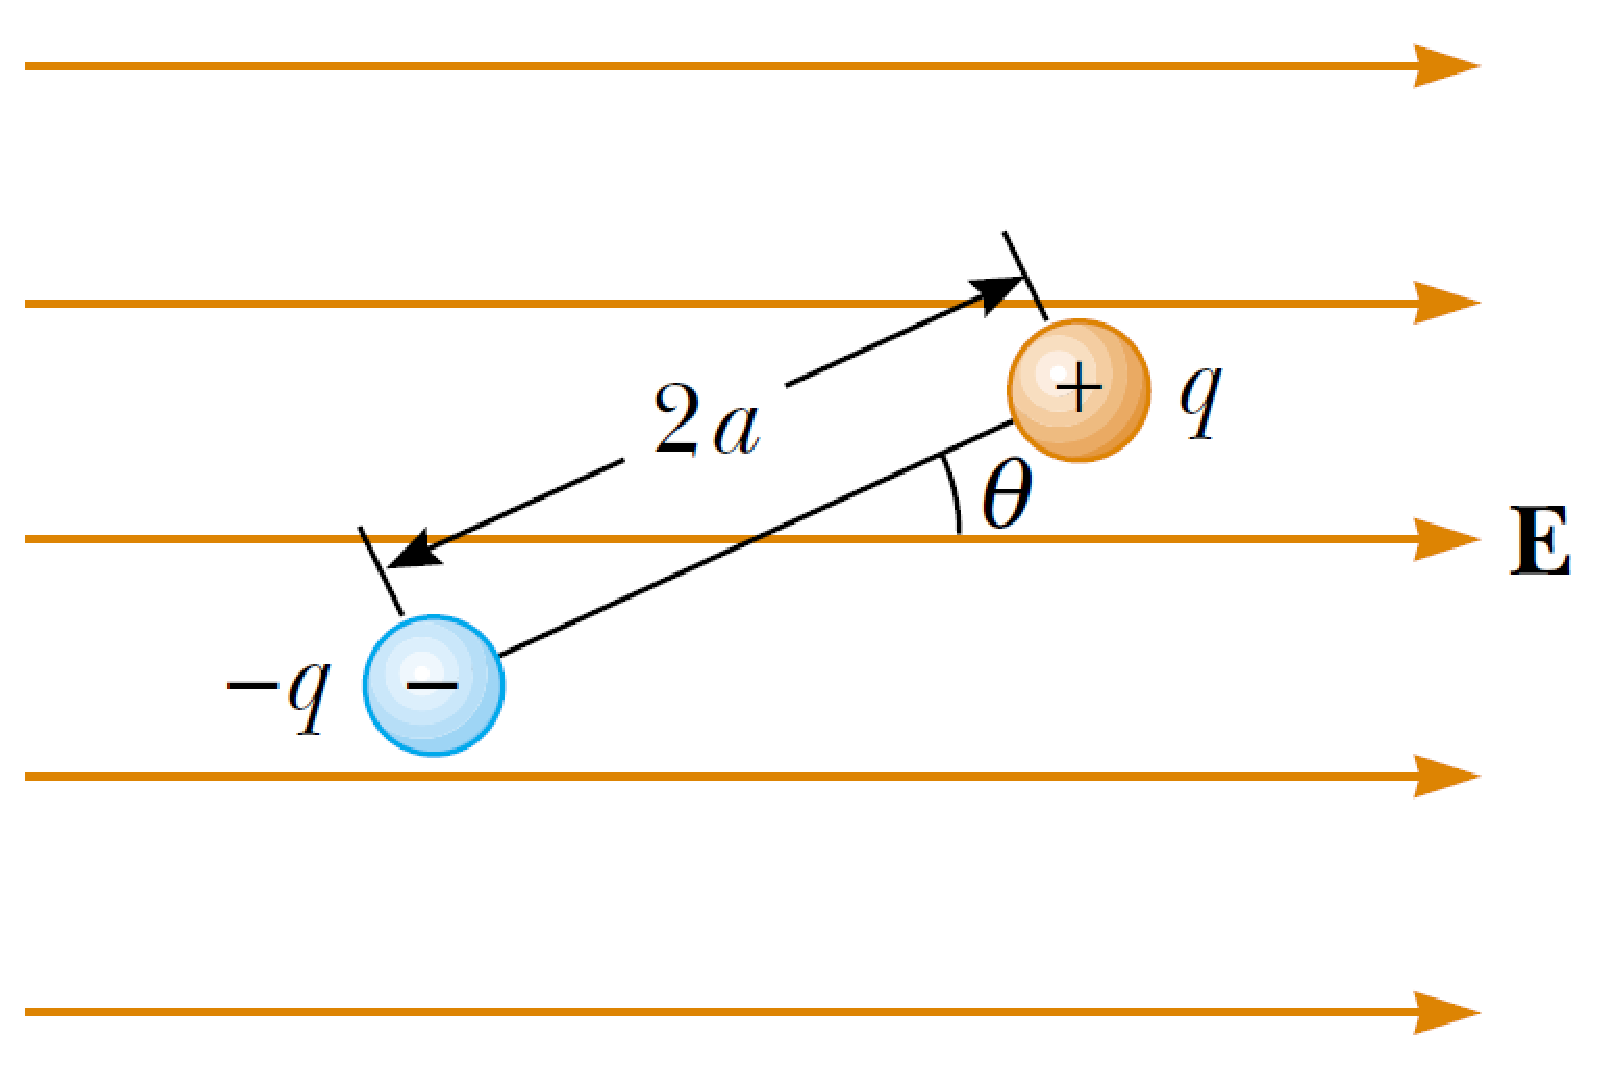
\includegraphics[scale=0.2]{MAS-dipolo}
\end{center}
}

\item Un electr�n entra a la regi�n de un campo el�ctrico uniforme $E=200$ N/c. 
Su rapidez de entrada es $v_{i}=3.0 \times 10^6$ m/s. La longitud horizontal de la placa es $l=10$ cm.

\begin{center}
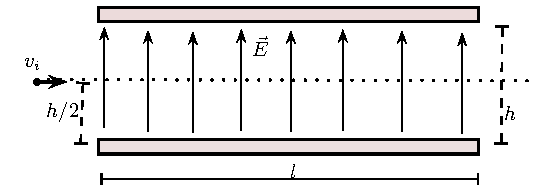
\includegraphics[scale=0.9]{capacitor}
\end{center}

\begin{enumerate}
\item Encuentre la aceleraci�n del electr�n mientras est� entre las placas.
\item �Cu�l debe ser la m�nima separaci�n $h$ de las placas para que el electr�n salga de ellas?
\end{enumerate}

\item Protons are projected with a inicial speed $v_i=9.55\times 10^3$ m/s into a region where a uniform electric field $\vec{E}=-720 \hat{j}$ N/C is present, as shown in figure. 
The protons are to hit a target that lies at a horizontal distance of $1.27$ mm from the point where the protons cross the plane and enter the electric field.

\begin{center}
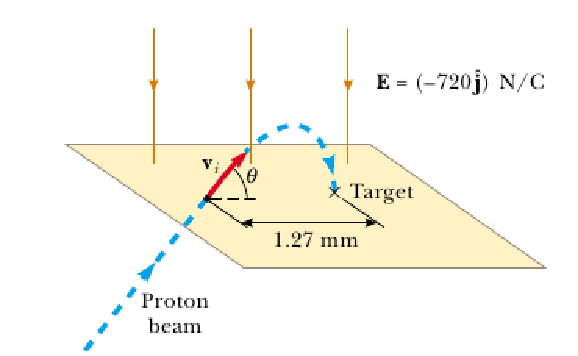
\includegraphics[scale=0.8]{tiro}
\end{center}

\begin{enumerate}
\item Find the angle $\theta$ shown in the figure. �Is there only one angle?
\item Find the total time of flight.
\end{enumerate}

\end{enumerate}
\end{document}
